\documentclass[a4paper,11pt]{article}
\usepackage{t1enc}
\usepackage[space]{grffile}
\usepackage[round, longnamesfirst]{natbib}  % Bindet den natbib-standard fuer das Zitieren ein
\usepackage{epsfig}
\usepackage{chngcntr}
\usepackage[latin1]{inputenc}   % Ermoeglicht Sonderzeichen direkt einzugeben
\usepackage[T1]{fontenc}        % Garantiert saubere Worttrennung bei Umlauten etc.
\usepackage{color}              % Farbpaket
\usepackage{amsmath,amsfonts,amssymb}   % ermoeglicht mathematische Sonderzeichen
\usepackage[english]{babel}     %
\usepackage{ae}                 %
\usepackage{graphicx}
\usepackage{longtable}          % zum erstellen von Tabellen ber mehrere Seiten
\usepackage{multirow}           % zum Verbinden von Zeilen innerhalb einer Tabelle
%\usepackage{pictexwd}           % PicTex, ein Graphikpaket
\usepackage{pst-all, multido}   % psTricks, ein Graphikpaket
\usepackage{url}
\usepackage[doublespacing]{setspace}
\usepackage{booktabs,caption,fixltx2e,array,dcolumn}
\usepackage{parskip}
\usepackage{etoolbox}
\usepackage{tabularx}
\usepackage{caption}
\usepackage{subcaption}
%\usepackage{morefloats}
\usepackage[section]{placeins} % Mit FloatBarrier kann verhindert werden, dass Float in der nächsten Section angezeigt werden
\usepackage[bottom]{footmisc} % Fußnoten werden ganz unten angezeigt
\setcitestyle{authoryear, open={((},close={))}}

\newcolumntype{L}[1]{>{\raggedright\arraybackslash}p{#1}} % linksbündig mit Breitenangabe
\newcolumntype{C}[1]{>{\centering\arraybackslash}p{#1}} % zentriert mit Breitenangabe
\newcolumntype{R}[1]{>{\raggedleft\arraybackslash}p{#1}} % rechtsbündig mit Breitenangabe

\makeatletter
\interfootnotelinepenalty 10000
\patchcmd{\Ginclude@eps}{"#1"}{#1}{}{}
\makeatother

\makeatletter
\newcommand\tageq{%
  \ifmeasuring@\else
    \refstepcounter{equation}%
  \fi
  \tag{\theequation}%
}
\makeatother

\newcommand\fnote[1]{\captionsetup{font=tiny}\caption*{#1}}

%\parindent 0cm
%\renewcommand{\baselinestretch}{1}

\renewcommand{\bibnumfmt}[1]{#1.}
\bibpunct{(}{)}{;}{a}{,}{,}

%%%%%%%%%%%%%%%%%%%%%%%%%%%%%%%%%%%%%%%%%%%%%%%%%%%%%%%%%%%%%%%%%%%%%%%%%%%%%%%%%%%%%%%%%%%%%%%%%%%%%%%%%%%%%%%%%%%%%%%%%%%%%%%%%%%%


% ________________ EINRICHTEN DES DOKUMENTS ______________________%

%\bibliographystyle{plainnat}    % legt den Stil fuer das Inhaltsverzeichnis fest

\oddsidemargin 0.0in \evensidemargin 0.0in \textwidth 15.5cm \topmargin -0.8in \textheight 24.5cm
\setlength{\parskip}{1pt}
\setlength{\parindent}{0pt}
\renewcommand{\baselinestretch}{1}


\setlength{\intextsep}{0.5cm} % Legt den Abstand zwischen Gleitobjekten und dem darüber und darunter angeordneten Fließtext fest.

%\oddsidemargin 0.1in \evensidemargin 0.1in \textwidth 15.5cm \topmargin -0.4in \textheight 24.5cm
%\parindent 0cm      % legt die Seitenraender fest

\pagestyle{plain}          % leere Kopfzeile, Seitennummer in der Mitte der Fusszeile

\newcommand{\bs}{\boldsymbol}  % shortcut zur Erzeugung von fetten Sympolen in der Mathe-Umgebung

%\renewcommand{\baselinestretch}{1.25}
% 1,5 -facher Zeilenabstand (Standard ist 1,2-facher Zeilenabstand, also 1,2*1,25 = 1,5

\begin{document}

\pagenumbering{roman}   % roemische Zahlen zur Seitennumerierung


%%%%%%%%%%%%%%%%%%%%%%%%%%%%%%%%%%%%%%%%%%%%%%%%%%%%%%%%%%%%%%%%%%%%%%%%%%%%%%%%%%%%%%%%%%%%%%%%%%%%%%%%%%%%%%%%%%%%%%%%%%%%%%%%%%%%%%%5


\begin{titlepage}       % Umgebung fuer Titelseite, frei gestaltbar

\thispagestyle{empty}   % keine Numerierung auf Titelseite

\begin{center}

\includegraphics[width=13cm]{Bild.png}
\end{center}

\begin{center}

\vspace*{1.5cm}
{\bf  \Large Assignment \#4: Option Valuation using Fourier Transform Methods} \\
\vspace*{2cm} 
\textbf{B473 Numerical Methods in Finance}
\\
Prof. Dr.-Ing. Rainer Sch\"obel
\\
\vspace*{0.5cm} 
Winter Term 2016-2017\\
\end{center}

\vfill
\begin{flushright}
    \emph{Konstantin Smirnov}\\
    \textit{Student-ID: 3980253}\\
     \textit{ Economics and Finance}\\
 T\"ubingen, \today
  




\end{flushright}



% 
% \begin{center}
% $ $			% oeffnet und schliesst eine Matheumgebung (Trick, um den Titel nach unten zu rutschen
% \vspace{4cm}
% 
% {\LARGE TITEL}
% \vskip 4cm
% 
% Diese Seite ist frei gestaltbar
% \end{center}

\end{titlepage}

\newpage                % erzwingt an dieser Stelle einen Seitenumbruch

\listoffigures
\newpage


\tableofcontents

\newpage
\pagenumbering{arabic}      % Seitenzahlen wieder arabisch numerieren
\setcounter{page}{1}        % Ruecksetzen des Seitenzahlzaehlers auf 1
\section{Introduction}
The Fourier-Inversion technique (FIT) is an alternative numerical method to solve for the probabilities of the option prices. The idea can be briefly described as follows: First we transform our PDE problem into the complex space via \textit{Fourier Transformation}. In the \textit{Fourier} space the problem can be solved analytically. Once we achieved a complex solution or \textit{characteristic function} of this problem, it can be solved numerically via the \textit{inverse Fourier transformation} in the real space. A great improvement of the FIT is that once you have a characteristic function, the PDE can be solved numerically. Hence this method is more flexible regarding different distributions as long as you can achieve a characteristic function.

In this paper we will examine how the FIT can be implemented for the classic Black-Scholes-Merton (BSM) case, as well for a modified Heston Model with stochastic volatility of Sch\"obel and Zhu (1999). We will analyse accuracy and efficiency of the FIT for both models and technical problems which can occur. Besides this, every chapter discusses technical implementation in \textit{MATLAB} at the end of each chapter.
\section{Black-Scholes-Merton model by Fourier Inversion}
In this section we will analyse how the FIT can be used and implemented in order to solve for a European Call option modeled in the standard BSM framework. 
\subsection{Theoretical Framework}
The BSM price of a European Call is defined as follows (Sch\"obel, 2017):
\begin{equation}
C_{Fourier}(S,t)= Sexp(h-r)F_1 - Kexp(-r(T-t))F_2
\label{BSMF}
\end{equation}
where we are interested in the risk-neutral probabilities $F_1$ and $F_2$.

First, in order to get the characteristic function, we use a Fourier transform:
\begin{equation*}
f(\phi)= \int_{-\infty}^{+\infty}e^{i\phi x} q(x)dx
\end{equation*}
where q(x) of Gaussian density
\begin{equation*}
q(x) = \dfrac{1}{v\sqrt{2\pi}} exp\left(-\dfrac{1}{2}(\dfrac{x-m}{v})^2\right)
\end{equation*}
with
\begin{eqnarray*}
x&=&ln S_T\\
m&=& ln S_T + (r - \dfrac{1}{2} \sigma^2)(T-t)\\
v^2&=&\sigma^2 (T-t)
\end{eqnarray*}
Substituting and completing the square of the complex function leads to the following characteristic functions:
\begin{equation}
f(\phi)_{1,2}=exp \{i\phi ln S - \dfrac{1}{2} \phi^2 \sigma^2 (T - t) + i \phi (r \pm \dfrac{1}{2} \sigma^2\ (T - t) \}
\label{cf}
\end{equation}
Equation (\ref{cf}) with respect to the inversion theorem leads to the risk-neutral probabilities $F_1$ and $F_2$ which can be now solved numerically:
\begin{equation}
F_{1,2}=\dfrac{1}{2}+\dfrac{1}{\pi}\int_0^{\infty} \! Re\left(\dfrac{exp\{-i\phi ln K\}}{i\phi} f_j(\phi) \right) \, \mathrm{d}\phi.
\label{CDF}
\end{equation}
It should be made clear that in order to integrate with the trapezoidal rule, the parameter $\phi$ plays a major rule regarding accuracy of the computation since it ''discretizes'' the continuous probability function into equally large parts, depending of the size of the $\phi$. Therefore this parameter consist of equally large intervals (''step-size'') with a range of $\epsilon$, a number really close to 0, to a given $\phi_{max}$. This will be discussed in more detail in the following chapter.
\subsection{Discussion of Results}
In this section several computations with a Fourier transform were calculated in order to compare accuracy and efficiency of FIT for varying $\phi_{max}$

In order to check accuracy, we assume the standard BSM closed-form solution as our benchmark. The standard BSM closed form solution for a European Call option is defined as:
\begin{equation}
C_{BCSM}(S,t)=S e^{(h-r)(T-t)}N(d_1)-Xe^{-r(T-t)}N(d_2)
\label{BCSM}
\end{equation}
with
\begin{equation*}
d_1=\frac{ln(\frac{S_t}{X})+(h+0.5\sigma^2)(T-t)}{\sigma \sqrt{T-t}}
\end{equation*}
\begin{equation*}
d_2=d_1-\sigma\sqrt{T-t}
\end{equation*}
With respect to (\ref{BSMF}) and (\ref{BCSM}), we compute the model error for varying $\phi_{max}$ as follows:
\begin{equation*}
\epsilon= C_{BSMC} - C_{Fourier}
\end{equation*}

Following sample parameters were used to value the price of a European Call option:

\begin{table}[!h]
\centering
\caption{Sample parameters of problem 1}
\begin{tabular}{l|l|l}
\textbf{Description} & \textbf{Variable} & \textbf{Value}  \\\hline
 stock price& S  & [100:1:300]  \\
 strike& K  & 210 \\
 Time to maturity& T - t  & 0.75 \\
 risk-free interest rate& r & 0.03 \\
 continuous dividend yield& q & 0.05  \\
 volatility& $\sigma$ & 0.3 
\end{tabular}
\end{table}

Our computations for different stock prices and $\phi_{max}$ and to the input parameters leads to following results shown in table \ref{result1}. As you can clearly see the error decreases with increasing $\phi_{max}$ since the integration area of the Fourier inverse is ''sliced'' into smaller parts while integrating. Note that in our calculation we used a $\phi$ size of 0.0001. Instead of varying the $\phi_{max}$ size, one could decrease the step-size of the interval which would lead to the  similar results as an increase in $\phi_{max}$. 
\newpage
\begin{table}[!h]
\caption{Model errors $\epsilon$}
\label{result1}
\begin{subtable}{.22\linewidth}
      \centering
        \caption{$\phi_{max}$=5}
\begin{tabular}{l|l}
 \textbf{S} & \textbf{$\epsilon$}  \\\hline
  100 & -2,9898\\
 200  &3,8046  \\
 300 & -0,1056 \\
\end{tabular}
\end{subtable}
\begin{subtable}{.22\linewidth}
      \centering
        \caption{$\phi_{max}$=10}
\begin{tabular}{l|l}
 \textbf{S} & \textbf{$\epsilon$}  \\\hline
  100 &0,04222   \\
 200  &0,1521  \\
 300 &-0,2276  \\
\end{tabular}
\end{subtable}
\begin{subtable}{.22\linewidth}
      \centering
        \caption{$\phi_{max}$=25}
\begin{tabular}{l|l}
 \textbf{S} & \textbf{$\epsilon$}  \\\hline
  100 & 1,0804e-09\\
 200 & -4,9056e-11   \\
 300 &-1,243e-09  \\
\end{tabular}
\end{subtable}
\begin{subtable}{.22\linewidth}
      \centering
        \caption{$\phi_{max}$=50}
\begin{tabular}{l|l}
 \textbf{S} & \textbf{$\epsilon$}  \\\hline
  100 &  2,2427e-14\\
 200  & 7,1054e-14 \\
 300 & -2,5580e-13 \\
\end{tabular}
\end{subtable}
\end{table}

Same findings can be found in figure (\ref{plot12}) where the stock price is plotted against the errors. Here we can also clearly see that increasing the number of $\phi_{max}$ increases accuracy. Specifically an increase from $\phi_{max}$=10 to $\phi_{max}$=25 improves it significantly, while an increase from $\phi_{max}$=25 to $\phi_{max}$=50 only marginally effects accuracy.

Another interesting fact can be observed while having a more detail look of the errors, represented in figure (\ref{plot13}). First of all, for increasing $\phi_{max}$, the error decreases whereas the volatility increases. What is more interesting is how the error develops for increasing S. The structure is similar to the development of the trigonometric functions which might come from the fact that the computed integral contains a real exponential function (\ref{CDF}). 
\begin{figure}[!h]
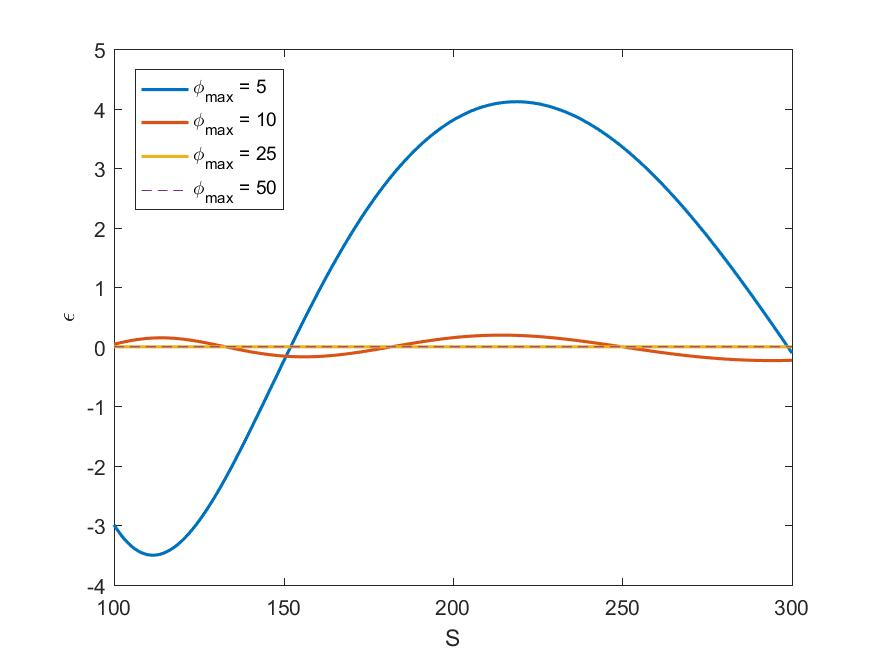
\includegraphics[width=12cm]{plot15.jpeg}
\centering
\caption{Fourier Inversion - BSM-Price Error for increasing $\phi_{max}$}
\label{plot12}
\end{figure}
\begin{figure}[!h]
\begin{subfigure}[c]{0.5\textwidth}
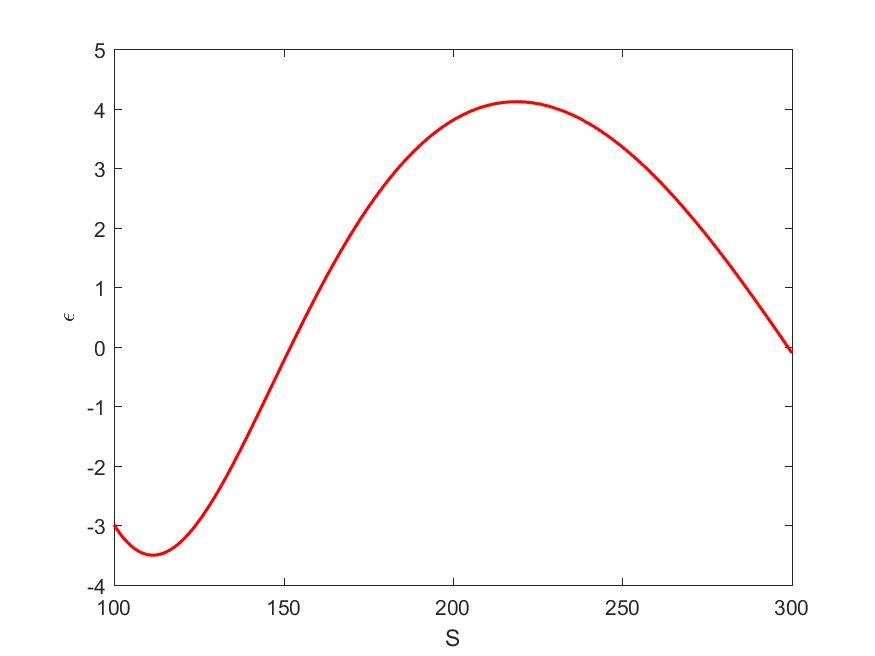
\includegraphics[width=8cm]{plot11.jpeg}
\subcaption*{$\phi_{max}$=5}
\end{subfigure}
\begin{subfigure}[c]{0.5\textwidth}
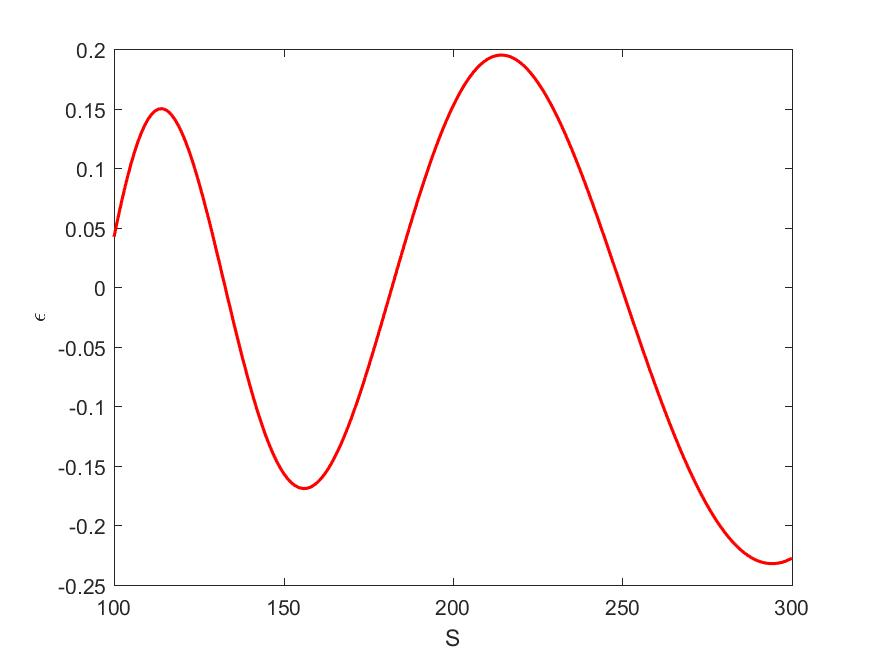
\includegraphics[width=8cm]{plot12.jpeg}
\subcaption*{$\phi_{max}$=10}
\end{subfigure}
\begin{subfigure}[c]{0.5\textwidth}
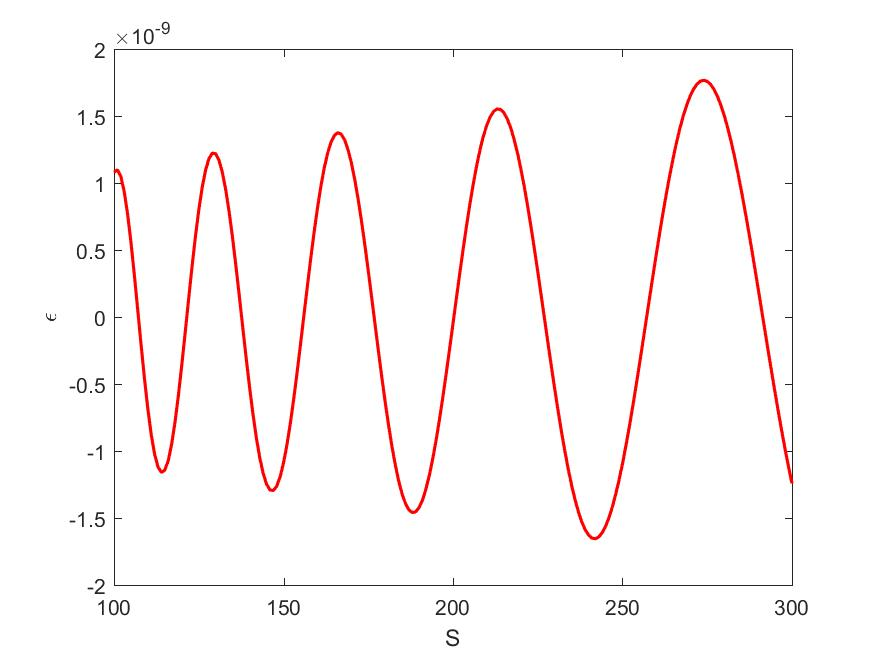
\includegraphics[width=8cm]{plot13.jpeg}
\subcaption*{$\phi_{max}$=25}
\end{subfigure}
\begin{subfigure}[c]{0.5\textwidth}
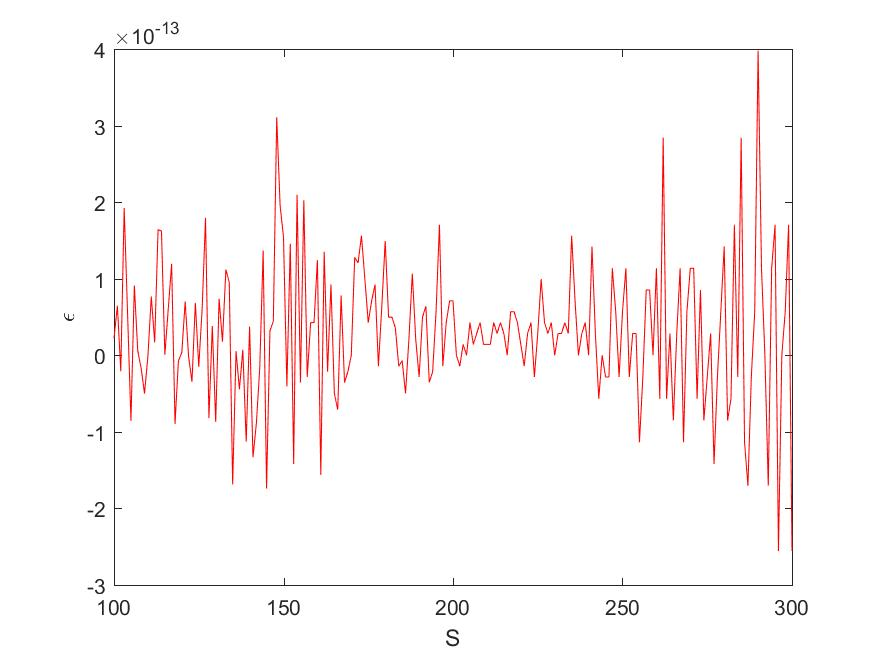
\includegraphics[width=8cm]{plot14.jpeg}
\subcaption*{$\phi_{max}$=50}
\end{subfigure}
\caption{Fourier Inversion - BSM-Price Error for increasing $\phi_{max}$ (in detail)}
\label{plot13}
\end{figure}

\begin{figure}[!h]
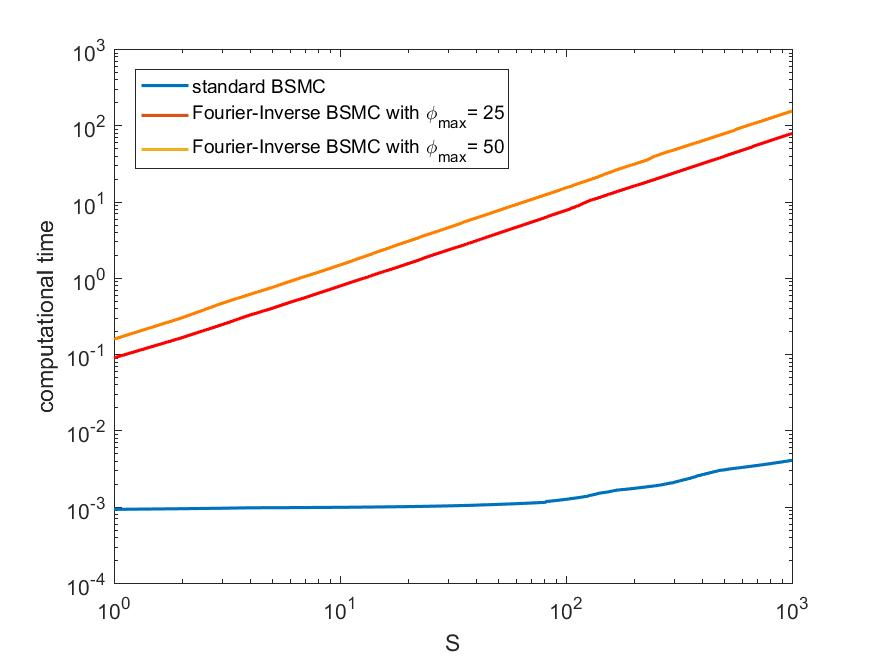
\includegraphics[width=11cm]{plot16.jpeg}
\centering
\caption{Fourier Inversion - Computational Time for S=200 (log-scaled)}
\label{plot16}
\end{figure}
\newpage

Figure (\ref{plot16}) shows the time efficiency of the FIT compared to the closed-form solution for 1000 runs and S=200 for a $\phi_{max}$=25 and $\phi_{max}$=50.\footnote{Note that time measure depends on the hardware of the computer and on the condition of the operation system. Hence time measures might be different from run to run.}. While the closed-form solution remains almost constant over time, the computational time of the FIT computations rise linearly with an increase in number of computations. While closed form-solutions needs only 0.0036 seconds, a FIT with $\phi_{max}$= 25 takes 76.8451 seconds, while a FIT computation with $\phi_{max}$= 50 doubles to 155.0175 seconds.

As we have seen above, an increase from $\phi_{max}$=25 to $\phi_{max}$= 50 only marginally improves the accuracy of the calculation but comes with doubled computational effort. Hence, as a suggestion for practical purposes, a $\phi_{max}$= 50 should not be favored due to time inefficiency. Instead a $\phi_{max}$ of around 20 should be the favorable choice, since it already delivers precise results for a relative efficient computational effort.

\subsection{Technical Implementation}
The computation and all necessary plots of problem 1 can be called in the main script \textit{Problem1.m}. In order to compute the European Call prices with FIT several connected functions were constructed with respect to the equations of the theoretical framework in section 2.1.

First one has to compute the characteristic functions which is obtained in script \textit{cfj.m}. It basically contains the characteristic function equation (\ref{cf}). The Fourier inversion process is stated in function \textit{InvIntegral.m}. Here equation (\ref{CDF}) is integrated (trapezoidal) with respect to the characteristic function and the parameter $\phi$ with help of the \textit{trapz} command to compute the probabilities $F_1$ and $F_2$. Finally the BSM price of the European Call with respect to equation (\ref{BSMF}) can be computed in the script \textit{BSMFourierInv.m} with respect to the given input parameters.

Since we are interested in different values for different stock prices and different $\phi$ levels, several loops were constructed. In order to compare the FIT prices with the theoretical ''real'' value for the call, we made use of a self written \textit{BSMC.m} function which contains the closed-form solution of the standard BSM model. 

To measure the computational time, the \textit{tic and toc}commands were used. In order to get a nice illustration, the measured time was accumulated for each run of the loop in which every accumulated time frame is saved as an own vector element.
 
Note that all computations were run on a Windows 10 64-bit operation system with an Intel(R) Core(TM) i7-5500U CPU 2.40 Ghz.
\section{A Stochastic Volatility Model}
One major weakness of the classic BSM model is the constant volatility assumption. Empirical research has shown that volatility itself changes for different strikes over time (''volatility smile'') which might lead to miss pricing.

There exist several models in order to face this problem. One famous FIT model is the Stein and Stein model (1991) in which the stochastic volatility follows mean reverting Ornstein-Uhlenbeck process with zero correlation. Sch\"obel and Zhu (1999) modified this model in which the correlation between instantaneous volatilities and the underlying stock returns is considered, which is the focus of this chapter. Besides this we will additionally discuss technical implementation problems which can occur using FIT (''Heston trap'').
\subsection{Theoretical Framework}
In the SZ model the stochastic process of the log of the stock price x(t) = ln S(t) and its instantaneous volatility v(t) can be described by
\begin{equation}
dx(t)=(r-\dfrac{1}{2}v^2 (t))dt + v(t) dW_s(t)
\label{s}
\end{equation}
\begin{equation}
dv(t)=\kappa(\theta - v(t))dt + \sigma dW_v(t)
\label{vola}
\end{equation}
where the Brownian motions $dW_s$ and $dW_v$ are correlated in the Sch\"obel and Zhu (1999) modification.
\begin{equation*}
\rho dt= dW_s(t) dW_v(t)
\end{equation*}
In order to get a closed-form solution of this model in the Fourier transform, we use the risk-neutral martingale measure \textit{Q} which leads to following price equation for a European Call option:
\begin{align*}
C(S,t,T)&=S(t) \mathbf{E}^{Q_1}[1_{x(T)>lnK}] - e^{-r(T-t)}K \mathbf{E}^{Q_2}[1_{x(T)>lnK}] \\
&= S(t) F^{Q_1}(S(T))>K) - e^{-r(T-t)}K F^{Q_2}(S(T))>K)
\end{align*}
As in chapter 2.1., we derive the corresponding characteristic function $f(\phi)_1$ and $f(\phi)_2$ to get the closed-form solution of the risk-neutral probabilities  $F^{Q_1}$ and  $F^{Q_2}$ in the Fourier-transform space. They are defined as:
\begin{align*}
C(S,t,T)&=S(t) \mathbf{E}^{Q_1}[1_{x(T)>lnK}] - e^{-r(T-t)}K \mathbf{E}^{Q_2}[1_{x(T)>lnK}] \\
&= S(t) F^{Q_1}(S(T))>K) - e^{-r(T-t)}K F^{Q_2}(S(T))>K)
\end{align*}
with respect to equations (\ref{s}) and (\ref{vola}) this leads to following characteristic functions $f_1(\phi)$ and $f_2(\phi)$:
\begin{equation}
\begin{split}
f_1(\phi)&=\mathbb{E}^Q[exp\{-r(T - t) - x(t) + (1+i\phi)x(T)\}] \\
&= exp\{ i\phi(r(T-t)+ x(t)) -\frac{1}{2}(1 + i\phi)rho[\sigma^{-1}v^2(t)+\sigma(T-t)]\} \\
&\cdot exp\{\frac{1}{2}D(t,T;s_1,s_3)v^2(t) +B(t,T;s_1,
s_2,s_3)v(t)+C(t,T;s_1,s_2,s_3)\}
\end{split} 
\label{cf21}
\end{equation} 
with the constants 
\begin{align*}
s_1 &= -\frac{1}{2}(1+i\phi)^2 (1-\rho^2)+ \frac{1}{2}(1+i\phi)(1-2\kappa\rho\sigma^{-1}) \\
s_2 &= (1+ i\phi)\kappa\theta\rho\sigma^{-1
} \\
s_3 &= \frac{1}{2}(1+i\phi)\rho\sigma^{-1}
\end{align*}
\begin{equation}
\begin{split}
f_2(\phi)&=\mathbb{E}^Q[exp\{i \phi x(T)\}] \\
&= exp\{i\phi(r(T-t)+x(t)) -\frac{1}{2}i\phi\rho[\sigma^{-1}v^2(t)+\sigma(T-t)]\} \\
&\cdot exp\{\frac{1}{2}D(t,T;\hat{s_1},\hat{s_3})v^2(t) +B(t,T;\hat{s_1},
\hat{s_2},\hat{s_3})v(t)+C(t,T;\hat{s_1},\hat{s_2},\hat{s_3})\}
\end{split}
\label{cf22}
\end{equation} 
with the constants 
\begin{align*}
\hat{s_1} &= \frac{1}{2} \phi^2 (1-\rho^2)+ \frac{1}{2} i \phi(1-2\kappa\rho\sigma^{-1}) \\
\hat{s_2} &= i\phi\kappa\theta\rho\sigma^{-1
} \\
\hat{s_3} &= \frac{1}{2} i\phi\rho\sigma^{-1}
\end{align*}

The auxiliary functions are given by:
\begin{equation}
\begin{split}
D(t,T)&=\frac{1}{\sigma^2}\left(\kappa - \gamma_1 \frac{sinh[\gamma_1(T-t)]+\gamma_2 cosh[\gamma_1(T-t)]}{cosh[\gamma_1(T-t)]+\gamma_2 sinh[\gamma_1(T-t)]}\right) \\ \\
B(t,T) &= \frac{1}{\sigma^2\gamma_1} \left(\frac{(\kappa\theta\gamma_1-\gamma_2 \gamma_3)+ \gamma_3(sinh[\gamma_1(T-t)] + \gamma_2 cosh[\gamma_1(T-t)])}{cosh[\gamma_1(T-t)] + \gamma_2 sinh[\gamma_1(T-t)]}-\kappa\theta\gamma_1 \right) \\ \\
C(t,T)&= -\frac{1}{2} ln(cosh[\gamma_1(T-t)] +\gamma_2 sinh[\gamma_1(T-t)])+\frac{1}{2}\kappa(T-t) \\ \\
&+ \frac{(\kappa^2\theta^2\gamma_1^{2} - \gamma_3^{2})}{2\sigma^2\gamma_1^{3}}\left(\frac{sinh[\gamma_1(T-t)]}{cosh[\gamma_1(T-t)]+\gamma_2sinh[\gamma_1(T-t)]}-\gamma_1(T-t)\right) \\ \\
&+ \frac{(\kappa\theta\gamma_1-\gamma_2\gamma_3)\gamma_3}{\sigma^2\gamma_1^{3}}\left(\frac{cosh[\gamma_1(T-t)]-1}{cosh[\gamma_1(T-t)]+\gamma_2 sinh[\gamma_1(T-t)]}\right)
\end{split}
\label{AXF}
\end{equation}
and the constants
\begin{align*}
\gamma_1=\sqrt{2\sigma^2s_1+\kappa^2}, \  \  \gamma_2=\frac{1}{\gamma_1}(\kappa-2\sigma^2s_3), \ \ \gamma_3=\kappa^2\theta-s_2\sigma^2
\end{align*}

Since we obtained now the characteristic functions (\ref{cf21}) and (\ref{cf22}), the risk-neutral probability distribution function  $F_1$ and $F_2$ can be computed in the same manner as we did in chapter 2.1. via Fourier Inversion:
\begin{equation}
F_{1,2}=\dfrac{1}{2}+\dfrac{1}{\pi}\int_0^{\infty} \! Re\left(\dfrac{exp\{-i\phi ln K\}}{i\phi} f_j(\phi) \right) \, \mathrm{d}\phi.
\label{CDF2}
\end{equation}
Finally this leads again to the pricing equation:
\begin{equation}
C(S,t)= SF_1 - Kexp(-r(T-t))F_2
\label{BSMVOLA}
\end{equation}
\newpage
\subsection{Sample Calculation}
In this subsection we compute the European Call price of the option with following parameters:

\begin{table}[h!]
\centering
\caption{Input parameters for problem 2}
\label{my-label}
\begin{tabular}{l|l|l}
\textbf{Description} & \textbf{Variable} & \textbf{Value}  \\\hline
 stock price& S  & 100  \\
 strike& K  & 95 \\
 Time to maturity& T - t  & 0.5 \\
 risk-free interest rate& r & 0.0953 \\
mean reversion parameter& $\kappa$ & 4.0  \\
 ''volatility of volatility''& $\sigma$ & 0.1 \\
  long-run volatility& $\theta$ & 0.3 \\
   correlation coefficient& $\rho$ & -0.5 \\
   instantaneous volatility of the stock price& v & 0.2 \\
\end{tabular}
\end{table}
\begin{table}[h!]
\caption{European Call prices in the SZ model}
\label{result2}
\centering
\begin{tabular}{l|l}
 \textbf{$\phi_{max}$} & \textbf{$C_{SZ}$}  \\\hline
  10 & 12.5463\\
 25  & 12.7513  \\
 50 & 12.7513 \\
\end{tabular}
\end{table}

The results are stated in table \ref{result2}. According to the assignment, the ''true value'' of the call price under the SZ Model is 12.751. For a small $\phi_{max}$ we get inaccurate results while, as suggested in section 2, for a $\phi_{max}$ = 25, our results are already accurate. Again, an increase on $\phi_{max}$ = 50 increases the accuracy only marginally and would come with higher computational effort. Note that the integral size of $\phi$ is 0.001.

\subsection{Correction of the ''Heston trap''}
As already discussed in the last assignment $\#$3 , we found out that in the SZ model, the FIT might deliver wrong probabilities for specific parameters.
In order to highlight the effect of the ''Heston trap'' and its correction, we choose unrealistically high parameters summarized in table \ref{input3}. The wrong value leads to a call price of 28.948 while the correct value should be 85.372.\footnote{In this calculation $\phi_{max}$ was set to 25 with a step-size of 0.001.}
\begin{table}[h!]
\centering
\caption{Input parameters for problem 2}
\label{input3}
\begin{tabular}{l|l|l}
\textbf{Description} & \textbf{Variable} & \textbf{Value}  \\\hline
 stock price& S  & 100  \\
 strike& K  & 120 \\
 Time to maturity& T - t  & 10 \\
 risk-free interest rate& r & 0.0953 \\
mean reversion parameter& $\kappa$ & 4.0  \\
 ''volatility of volatility''& $\sigma$ & 2.0 \\
  long-run volatility& $\theta$ & 0.5 \\
   correlation coefficient& $\rho$ & -0.8 \\
   instantaneous volatility of the stock price& v & 0.15 \\
\end{tabular}
\end{table}

\begin{figure}[!h]
\caption{Probability function $F_1$ and $F_2$ in the SZ model}
\begin{subfigure}[c]{0.5\textwidth}
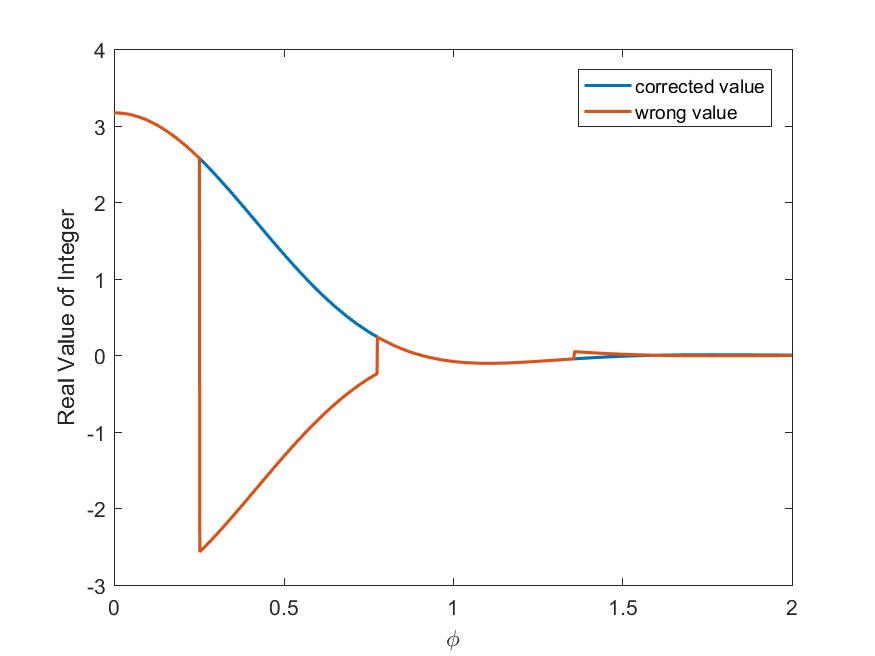
\includegraphics[width=8cm]{plot31.jpeg}
\subcaption*{$F_{1}$}
\end{subfigure}
\begin{subfigure}[c]{0.5\textwidth}
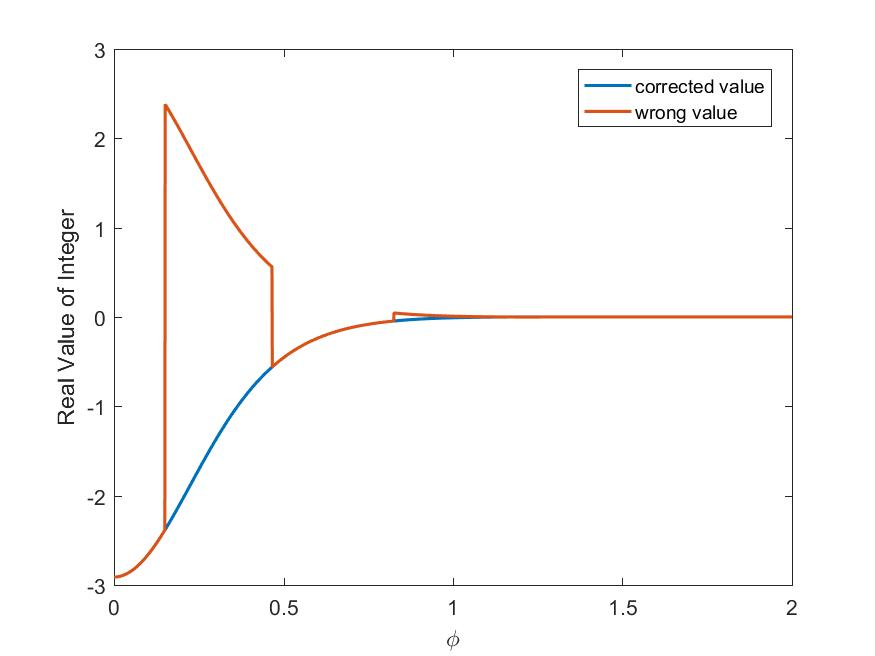
\includegraphics[width=8cm]{plot32.jpeg}
\subcaption*{$F_{2}$}
\end{subfigure}
\label{pl3}
\end{figure}
The problem arises from a technical issue \textit{MATLAB} faces when computing the complex logarithm of the auxiliary function C(t,T) in (\ref{AXF}).
This will be more clear if we have a closer look on the general function of a complex logarithm:
\begin{equation*}
Log z = ln|z| + i Arg z =   ln|z| + i (\varphi + i 2\pi k)
\end{equation*}
At some point the principal value reaches \textit{Arg}= $\pi$, or in other words, it reaches the negative real axis if z comes from the top. In that case, instead of increasing in $\pi$, it immediately jumps to -$\pi$ since, by definition, the principal value is only defined for (-$\pi$ $\pi$] which will lead to discontinuity in the probability function illustrated in figure \ref{pl3}. Same holds if z ''comes from the bottom''. Unfortunately, MATLAB does not take this into account while computing the principal value and which hence will lead to wrong result under these circumstances. 

To fix this issue, one can adjust the function in the following way (Sturm, 2017). If z crosses the real axis from above, one just simply increase the integer k of the principal value  by +1, while if z crosses the real axis from below, one simply decreases the integer k by -1. 

\subsection{Call Prices with Stochastic Volatility}
In this section we discuss several important finding of the SZ model regarding the instantaneous volatility v(t). For illustration of this discussion, figures \ref{41} and \ref{42} show different out-of-the money call prices for a $\theta$ of 0 and 0.2, respectively, with following parameters:
\begin{table}[h!]
\centering
\caption{Input parameters for problem 4}
\label{input3}
\begin{tabular}{l|l|l}
\textbf{Description} & \textbf{Variable} & \textbf{Value}  \\\hline
 stock price& S  & 100  \\
 strike& K  & 120 \\
 Time to maturity& T - t  & 3 \\
 risk-free interest rate& r & 0.0953 \\
  mean reversion parameter& $\kappa$ & 0.5  \\
 ''volatility of volatility''& $\sigma$ & 0.1 \\
   correlation coefficient& $\rho$ & [-1:0.1:1] \\
   instantaneous volatility of the stock price& v & [-0.6:0.1:0.6] \\
\end{tabular}
\end{table}

First of all, in the original model of Stein and Stein it is said that the instantaneous volatility v(t) in a mean-reverting OU process only enters as squared function v(t) into the model and hence should deliver symmetric prices for a negative or positive -v(t) / v(t). This assumption is graphically analyzed in figure \ref{41} and \ref{42}. But as it can be seen in those illustrations, this is only the case if $\theta$ is equal to 0 since symmetry disappears in figure 3. Hence the statement of Stein and Stein is not correct and v(t) does not enter in a squared fashion. More likely v(t) itself has an effect on the price of the option (Sch\"obel and Zhu, 1999).

\begin{figure}[!h]
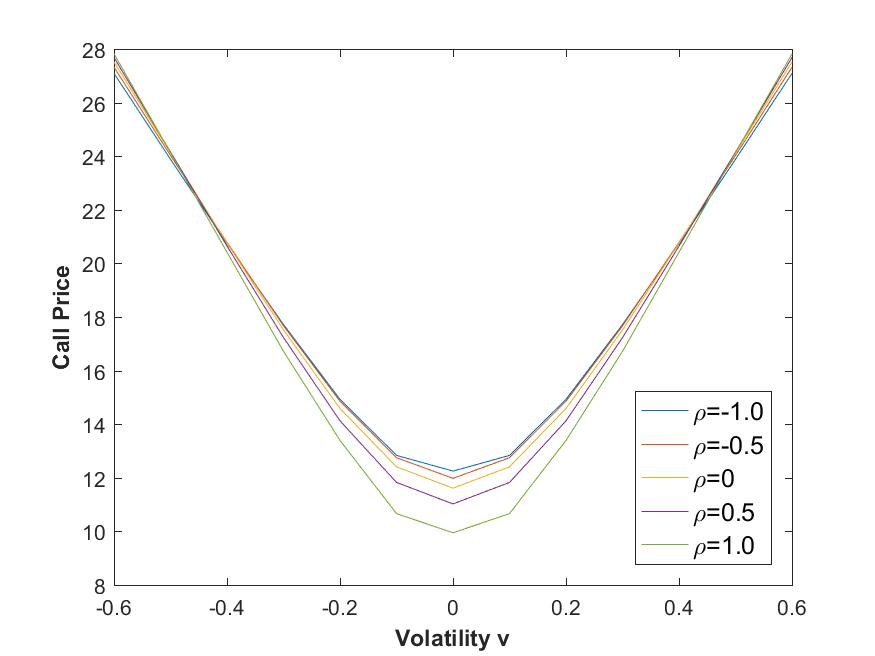
\includegraphics[width=12cm]{plot41.jpeg}
\centering
\caption{''Volatility Smile'' for $\theta$=0}
\label{41}
\end{figure}

\begin{figure}[!h]
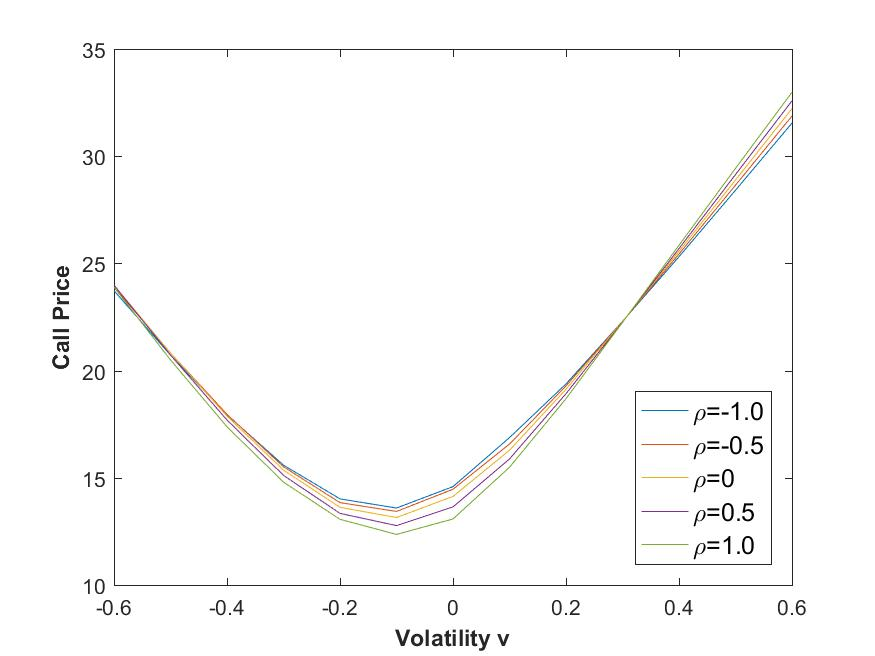
\includegraphics[width=12cm]{plot42.jpeg}
\centering
\caption{''Volatility Smile'' for $\theta$=0.2}
\label{42}
\end{figure}

Besides this, one can see following behavior for different combinations of v, $\rho$ and the out-of-the-money call price. First of all with increasing v(t) the call price in general increases since the value of an option always increases with increasing volatility.

What is more interesting is how the factor $\rho$ of the option comes into play. It is defined as the correlation between the stock price and the volatility of the option. For negative $\rho$ this means that an increase in S decreases the factor v(t) and vice versa.

In figure \ref{42} you can see that a negative correlation factor $\rho$ leads to higher call prices if v(t) is low. If we would consider decreasing stock prices under this regime, the positive effect of volatility on the call would "crowd out" the negative effect of the price due to an increase in S. On the other hand, if the stock price would rise, this would lead to a lower volatility v(t). But since the volatility is already low, the effect is relatively small.

On the other side, if v(t) is high, a negative correlation factor leads to relatively low call prices. If S would increase under this volatility regime, v(t) decreases while a decrease in S(t) would lead to a relative low price increase. In other words, the marginal effect of v(t) under this regime is relatively low since high volatility is already ''priced in'' due to the high volatility regime.

\subsection{Technical Implementation}
Problem 2, 3 and 4 of the assignment were implemented in the scripts \textit{Problem2.m}, \textit{Problem3.m} and \textit{Problem4.m}, respectively.
All of these scripts contain the main algorithm \textit{$SZ\_FourierInv.m$} which constructed basically in the same manner as the algorithms of the first problem, described in section 2.3., with respect to the theoretical equations described in the theoretical framework of this chapter. 

The Heston trap was simply corrected by using several \textit{if} statements which check if the z is crossing the real negative axis, and in case we just increase/decrease the counter variable k. Note that one can adjust the input parameter ''Heston'' for that case, in the function \textit{$SZ\_FourierInv.m$}. By setting it "1" one corrects the principal value.

\newpage
\section{References}
\

Sturm, Pascal. \textit{Assignment No. 3: Graphical Analysis of Characteristic Functions.} B473 Numerical Methods in Finance, T\"ubingen, 2017.
\\

Sch\"obel, Rainer and Jianwei Zhu. \textit{Stochastic Volatility With an Ornstein-Uhlenbeck Process: An Extension.} European Finance Review 3, 1999, 23 - 46.
\\

Sch\"obel, Rainer. \textit{B473 Numerical Methods in Finance}. Lecture Script, T\"ubingen, 2017.
\end{document}